\chapter{Parameter Estimation}
One of the most important ways of using Bayes' rule is in the topic
called {\it parameter estimation}. Parameter estimation is a fairly common
situation in statistics. In fact, it is possible to interpret almost any
problem in statistics as a parameter estimation problem and approach it
in this way!

Firstly, what is a parameter? Well, it is just a fancy term for a quantity or
a number that is unknown. For example, how many people are currently in New
Zealand? Well, a Google search suggests 4.405 million. But that does not mean
there are {\bf exactly} 4,405,000 people. It could be a bit more or a bit
less. Maybe it is 4,405,323, or maybe it is 4,403,886. We don't really know.
We could call the true number of people in New Zealand right now $\theta$, or
we could use some other letter or symbol if we liked.

The key is to realise that we can use the Bayes Box like in previous chapters,
but now, our list of possible hypotheses is a list of possible values for
the unknown parameter. For example, a Bayes Box for the precise number of
people in New Zealand might look something like this:
\begin{table}[h!]
\begin{center}
\begin{tabular}{|c|c|c|c|c|}
\hline
{\bf Possible Hypotheses} & {\tt prior} & {\tt likelihood} &
{\tt prior $\times$ likelihood} & {\tt posterior}\\
\hline
\ldots & \ldots & \ldots & \ldots & \ldots\\
$\theta = 4404999$ & 0.000001 & \ldots   & \ldots  & \ldots\\
$\theta = 4405000$ & 0.000001 & \ldots   & \ldots  & \ldots\\
$\theta = 4405001$ & 0.000001 & \ldots   & \ldots  & \ldots\\
$\theta = 4405002$ & 0.000001 & \ldots   & \ldots  & \ldots\\
$\theta = 4405003$ & 0.000001 & \ldots   & \ldots  & \ldots\\
$\theta = 4405004$ & 0.000001 & \ldots   & \ldots  & \ldots\\
$\theta = 4405005$ & 0.000001 & \ldots   & \ldots  & \ldots\\
$\theta = 4405006$ & 0.000001 & \ldots   & \ldots  & \ldots\\
\ldots & \ldots & \ldots & \ldots & \ldots\\
\hline
Totals: & 1 & & \ldots & 1\\
\hline
\end{tabular}
\end{center}
\end{table}
There are a few things to note about this Bayes' box. Firstly, that it is big.
There are lots of possible hypotheses, corresponding to possible values for
$\theta$. The prior probabilities I have put in the 2nd column were for
illustration purposes. 

\section{Parameter Estimation: Bus Example}
This is a beginning example of parameter estimation from a Bayesian point of
view. It shows the various features that are always present in a Bayesian
analysis: prior probabilities, likelihood, and posterior probabilities.

After moving to Auckland, I decided that I would take the bus to work
each day. However, I wasn't very confident with the bus system, so for the first
week I just took the first bus that came along and was heading in the right
direction (towards the city).

{\bf Here's the question}. In the first week, I caught 5 morning buses.
Of these 5 buses, two of them took me to the right place, while three of them
took me far from work, leaving me with an extra 20 minute walk. Given this
information, 




Discrete
Bayes Box

Bus example

\begin{table}
\begin{center}
\begin{tabular}{|c|c|c|c|c|}
\hline
\tt{Possible Values} & \tt{Prior} & \tt{Likelihood} & \tt{h} & \tt{Posterior}\\
$\theta$ & $P(\theta)$ & $P(x|\theta)$ & $P(\theta)P(x|\theta)$ & $P(\theta|x)$\\
\hline
0 & 0.0909 & & &\\
0.1 & 0.0909 & & &\\
0.2 & 0.0909 & & &\\
0.3 & 0.0909 & & &\\
0.4 & 0.0909 & & &\\
0.5 & 0.0909 & & &\\
0.6 & 0.0909 & & &\\
0.7 & 0.0909 & & &\\
0.8 & 0.0909 & & &\\
0.9 & 0.0909 & & &\\
1 & 0.0909 & & &\\
\hline
Totals & 1 & & & 1\\
\hline
\end{tabular}
\end{center}
\end{table}

Continuous?


\chapter{Parameter Estimation: Analytical Methods}
Analytical methods are those that can be carried out with a pen and paper,
the ``old school'' way before we all started using computers. There are some
problems in Bayesian statistics that can be solved in this way, and we will
see one or two of them in this course.

Let's look at the {\it binomial likelihood} problem again, with the familiar
bus example. Out of $N=5$ attempts at a ``repeatable'' experiment, there were
$x=2$ successes. From this, we want to infer the value of $\theta$, the
success probability that applied on each trial. Because of its meaning, we know
with 100\% certainty that $\theta$ must be between 0 and 1 (inclusive).

Recall that, if we knew the
value of $\theta$ and wanted to predict the data $x$ (regarding $N$ as being
known in advance), then we would use the binomial distribution:
\begin{eqnarray}
p(x|\theta) &=& \left(\begin{array}{c}N \\ x\end{array}\right)
\theta^x\left(1-\theta\right)^{N - x}.\label{eq:binomial_likelihood}
\end{eqnarray}
This is the probability mass function for $x$. Since there are five trials
($N=5$), the number of successes $x$ must be one of 0, 1, 2, 3, 4, or 5.
If $\theta$ is a high number close to one, then we would expect the resulting
value of the data $x$ to be something high like 4 or 5. Low values for $x$ would
still be possible but they would have a small probability. If $\theta$ is a
small number, we would expect the data to be 0, 1, or 2, with less probability
for more successes than that. This is just saying in words what is written
precisely in Equation~\ref{eq:binomial_likelihood}. The probability distribution
for the data $x$ is plotted in Figure~\ref{fig:binomial} for three illustrative
values of the parameter $\theta$.
\begin{figure}[h!]
\begin{center}
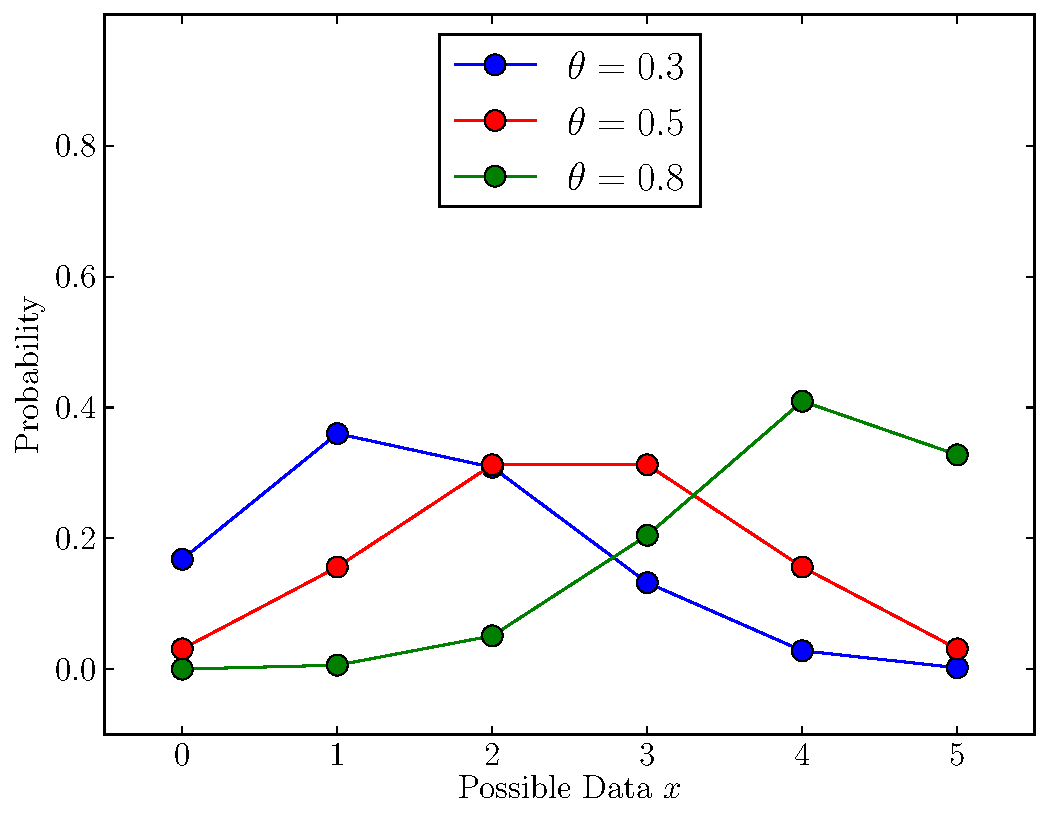
\includegraphics[scale=0.6]{Figures/binomial.pdf}
\caption{\label{fig:binomial}}
\end{center}
\end{figure}


